\section{Specifications}


\begin{table}[htbp]
\label{motor_specs}
\caption[Specifications of supported motors.]{Specifications of supported motors.}
\centering
\begin{tabular}{|l|c|c|}
\hline 
 & SMC2242 & SMC4242 \\ \hline 
Number of Motors: & 2 & 4 \\ \hline
Motor Type: & \multicolumn{2}{c|}{Bipolar Stepper Motor} \\ \hline
Motor Drive Voltage: & \multicolumn{2}{c|}{\unit[24]{V}} \\ \hline
Motor Current: & \multicolumn{2}{c|}{up to \unit[2.5]{A} peak or \unit[1.75]{A} RMS} \\ \hline
\end{tabular}
\end{table}


\begin{table}[htbp]
\label{features_of_versions}
\caption[Features of different versions.]{Features of different versions.}
\centering
\begin{tabular}{|l|c|c|c|}
\hline 
 & SMCx242-R & SMCx242-L & SMCx242-U \\ \hline 
Units: & $\degree$, $\pi$, steps & m, cm, mm, steps & $\degree$, $\pi$, m, cm, mm, steps, user-defined \\ \hline
Substeps: & \multicolumn{3}{c|}{1, 2, 4, 8, 16, 32} \\ \hline
Steps per Revolution: & \multicolumn{3}{c|}{200, 400} \\ \hline
Gear Ratio: & \multicolumn{3}{c|}{???} \\ \hline
Reference/Limit Switches: & 1 & \multicolumn{2}{c|}{3} \\ \hline
\end{tabular}
\end{table}


\begin{table}[htbp]
\label{motor_specs}
\caption[Technical Specifications.]{Technical Specifications.}
\centering
\begin{tabular}{|l|c|}
\hline 
Power requirements: & ? \\ \hline 
Power consumption: & \unit[]{W} \\ \hline 
Dimensions: & \unit[245]{mm} (W) x \unit[85]{mm} (H) x \unit[260]{mm} (D) \\ \hline 
Weight (without package): & \unit[]{kg} \\ \hline 
\end{tabular}
\end{table}



\section{Pinout}
The connectors for the stepper motors are 9-Pin D-Type, female connectors. Please refer to figure~\ref{pin_out} for their pinout.

\begin{figure}[h]
\begin{center}
\begin{minipage}[h]{5cm}
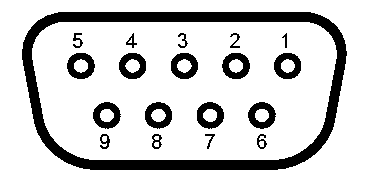
\includegraphics[width=5cm]{grafiken/Numbered_DE9_female_Diagram.pdf}
\end{minipage}
%\hspace{1cm}
\hfill
\begin{minipage}[h]{5cm}
\begin{tabular}{|c|c|}
\hline 
\textbf{Pin} & \textbf{Description} \\ \hline 
1 & Bridge B output 1 \\ \hline 
2 & Bridge B output 2 \\ \hline 
3 & Bridge A output 2 \\ \hline 
4 & Bridge A output 1 \\ \hline 
5 & Ground \\ \hline 
6 & \unit[+5]{V} \\ \hline 
7 & Reference/Limit Switch 1 \\ \hline 
8 & Reference/Limit Switch 2 \\ \hline 
9 & Reference/Limit Switch 3 \\ \hline 
\end{tabular}
\end{minipage}
\end{center}
\caption[Pinout of the Motor Connector.]{Pinout of the Motor Connector.}
\label{pin_out}
\end{figure}










\newpage
